% Build with XeLaTeX. The cover follows the supplied PTIT report template.
\documentclass[12pt,a4paper,oneside]{report}
\usepackage{fontspec}
\setmainfont{Times New Roman}
\setsansfont{Arial}
\usepackage[margin=22mm,headheight=16pt]{geometry}
\usepackage{graphicx}
\usepackage{eso-pic}
\usepackage{booktabs}
\usepackage{tabularx}
\usepackage{array}
\usepackage{fancyhdr}
\usepackage{hyperref}
\usepackage{xurl}
\usepackage{microtype}
\graphicspath{{assets/}}
\hypersetup{
  hidelinks,
  pdftitle={From Analysis to Design: MVC and DAO Class Design for E-Commerce},
  pdfauthor={Vu Dinh Hieu},
  pdfsubject={Academic report on a Visual Paradigm e-commerce class diagram}
}
\pagestyle{fancy}
\fancyhf{}
\fancyhead[L]{E-Commerce System Design}
\fancyhead[R]{B23DCCE036}
\fancyfoot[C]{\thepage}
\setlength{\parindent}{1cm}
\setlength{\parskip}{4pt}
\setlength{\emergencystretch}{2em}
\renewcommand{\arraystretch}{1.18}
\newcolumntype{Y}{>{\raggedright\arraybackslash}X}

\begin{document}
\begin{titlepage}
\AddToShipoutPictureBG*{\AtPageLowerLeft{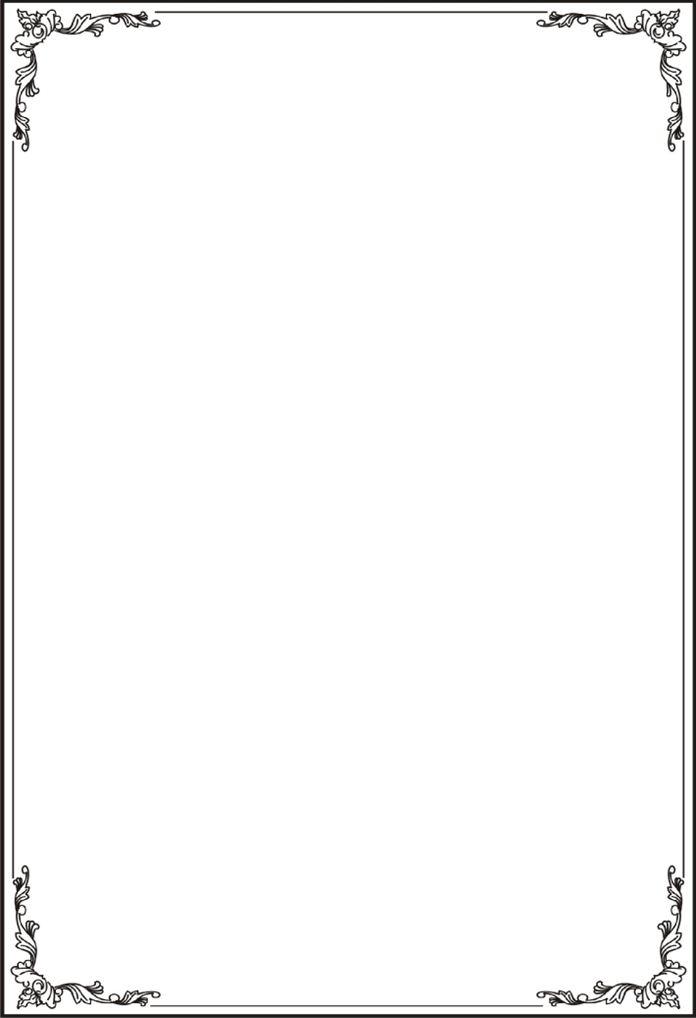
\includegraphics[width=\paperwidth,height=\paperheight]{assets/background.png}}}
\centering
\vspace*{10mm}
{\large\bfseries POSTS AND TELECOMMUNICATIONS\par}
{\large\bfseries INSTITUTE OF TECHNOLOGY\par}
\vspace{2mm}
{\normalsize\bfseries FACULTY OF INFORMATION TECHNOLOGY 1\par}
\vspace{10mm}

\includegraphics[width=30mm]{assets/logo.png}\par
\vspace{16mm}
{\Large\bfseries ACADEMIC DESIGN REPORT\par}
\vspace{7mm}
{\Huge\bfseries FROM ANALYSIS\par}
\vspace{2mm}
{\Huge\bfseries TO DESIGN\par}
\vspace{6mm}
{\large MVC and DAO Class Design for an E-Commerce System\par}
\vspace{17mm}
\rule{0.68\textwidth}{0.5pt}\par
\vspace{8mm}
\begin{minipage}{0.76\textwidth}
\large
\setlength{\parindent}{0pt}
\begin{tabular}{@{}p{47mm}>{\raggedright\arraybackslash}p{70mm}@{}}
Student: & \textbf{Vu Dinh Hieu}\\[3mm]
Student ID: & \textbf{B23DCCE036}\\[3mm]
Design artifact: & \textbf{eComDesign.vpp}\\[3mm]
Course topic: & \textbf{Information Systems Analysis and Design}
\end{tabular}
\end{minipage}\par
\vfill
{\normalsize September 2026\par}
\vspace*{8mm}
\end{titlepage}

\pagenumbering{roman}
\chapter*{Abstract}
\addcontentsline{toc}{chapter}{Abstract}
This report documents the transition from an analysis-oriented e-commerce class model to a layered object-oriented design. The resulting Visual Paradigm artifact organizes the system into a presentation interface, controllers, and domain model. Data access is expressed through DAO interfaces and repository implementations, allowing controllers to depend on contracts rather than persistence details. The design addresses four principal functional areas: customer management, shopping carts, item catalog browsing, and order processing. The final class diagram is included as the central design artifact and is interpreted through responsibilities, dependencies, and representative interaction paths.

The report also distinguishes structural verification from executable validation. The project was opened and exported with Visual Paradigm; the final diagram contains 35 class shapes, no overlapping class rectangles within the same package, and no broken diagram connector references. These checks establish that the edited artifact is structurally coherent and readable. They do not constitute a running Spring application or a proof of all business rules.

\noindent\textbf{Keywords:} e-commerce; UML class diagram; MVC; Data Access Object; layered architecture; analysis-to-design transformation.

\tableofcontents
\clearpage
\pagenumbering{arabic}

\chapter{Introduction}
\section{Problem context}
An analysis model identifies domain concepts and their relationships. A design model must additionally assign software responsibilities, make dependencies explicit, and define boundaries between interaction, business state, and persistence. In the supplied course handout, the e-commerce system is used to demonstrate this progression: methods are added to classes, selected associations are replaced by use dependencies, DAO interfaces are introduced, and the classes are organized into an MVC-oriented architecture~\cite{handout}.

The design presented here is a class-level view of that progression. It is intended to communicate how the e-commerce application could be structured, rather than to prescribe a database schema or claim that a deployed application already exists. The diagram is maintained in the editable Visual Paradigm project \texttt{eComDesign.vpp}; Figure~\ref{fig:mvc} reproduces its final exported view.

\section{Objectives and scope}
The objectives are to separate presentation from domain data, place request coordination in controllers, provide explicit persistence contracts for the main aggregates, and retain traceability to the original customer, cart, order, and item concepts. The scope of this report is the UML design artifact and its architectural interpretation. Operational concerns such as authentication, payment-provider integration, transactional behavior, and deployment are identified as further design work rather than silently assumed to be complete.

\chapter{Design Foundations}
\section{From analysis classes to design classes}
In analysis, a class can be understood primarily as a business concept. In design, its operations and dependencies must express a realizable responsibility. For example, a \texttt{Cart} stores cart state and exposes operations related to adding or removing items and calculating a total. A controller coordinates the request that invokes those operations, while a DAO retrieves or saves the corresponding data. This allocation prevents a single class from carrying user-interface, business, and persistence responsibilities simultaneously.

The handout distinguishes methods intrinsic to an object from methods that use another class~\cite{handout}. UML use dependencies in the design therefore indicate that one element requires another element's public contract. They should not be interpreted as database foreign keys or as proof of a complete runtime call sequence. Associations and inheritance remain appropriate where the domain relationship itself is the information being represented.

\section{MVC and DAO}
The Model--View--Controller pattern divides interaction into complementary concerns. A view presents information and accepts user input; a controller receives or coordinates a user action; the model represents domain state and rules. The diagram's \texttt{interface (view)}, \texttt{controller}, and \texttt{model} packages make these responsibilities visible. In an implementation, a controller may call a view method to present a result, while user events enter the system through the interface. A static class diagram expresses dependencies between classes, not the temporal ordering of every event.

The Data Access Object pattern places persistence operations behind an interface such as \texttt{CustomerDAO}, \texttt{CartDAO}, \texttt{ItemDAO}, or \texttt{OrderDAO}. Repository classes implement these contracts. This arrangement makes the controller's required data operations explicit and permits a persistence mechanism to change without making the controller dependent on a specific storage API. The DAO abstraction concerns access to domain objects; it does not replace domain behavior in \texttt{Cart}, \texttt{Order}, or \texttt{Item}.

\begin{table}[htbp]
\centering
\caption{Responsibilities represented by the design layers.}
\begin{tabularx}{\textwidth}{@{}>{\raggedright\arraybackslash}p{38mm}Y Y@{}}
\toprule
Layer or role & Principal responsibility & Representative classes \\
\midrule
Interface (view) & Display data and expose user-facing actions. & \texttt{CustomerView}, \texttt{CartView}, \texttt{ItemView}, \texttt{OrderView} \\
Controller & Coordinate requests and use data-access contracts. & \texttt{CustomerController}, \texttt{CartController}, \texttt{ItemController}, \texttt{OrderController} \\
DAO contract & Specify retrieval and persistence operations. & \texttt{CustomerDAO}, \texttt{CartDAO}, \texttt{ItemDAO}, \texttt{OrderDAO} \\
Repository implementation & Realize a DAO contract using a persistence component. & \texttt{CustomerDAOImpl}, \texttt{CartDAOImpl}, \texttt{ItemDAOImpl}, \texttt{OrderDAOImpl} \\
Domain model & Represent customer, catalog, cart, order, payment, and shipment state. & \texttt{Customer}, \texttt{Item}, \texttt{Cart}, \texttt{Order}, \texttt{Payment}, \texttt{Shipment} \\
\bottomrule
\end{tabularx}
\end{table}

\chapter{E-Commerce Class Design}
\section{Overview of the final diagram}
The design is arranged in three horizontal tiers. The upper package contains four views, each corresponding to a major user-facing area. The middle package contains four controller columns. Within each column, the controller, DAO interface, and repository implementation are vertically aligned so that their responsibilities can be compared directly. The lower \texttt{model} package contains the customer, order, and item subpackages. This layout preserves the project's original classes and relationships while making the principal layer boundaries easier to inspect.

\clearpage
\thispagestyle{plain}
\begin{figure}[htbp]
\centering
\makebox[\textwidth][c]{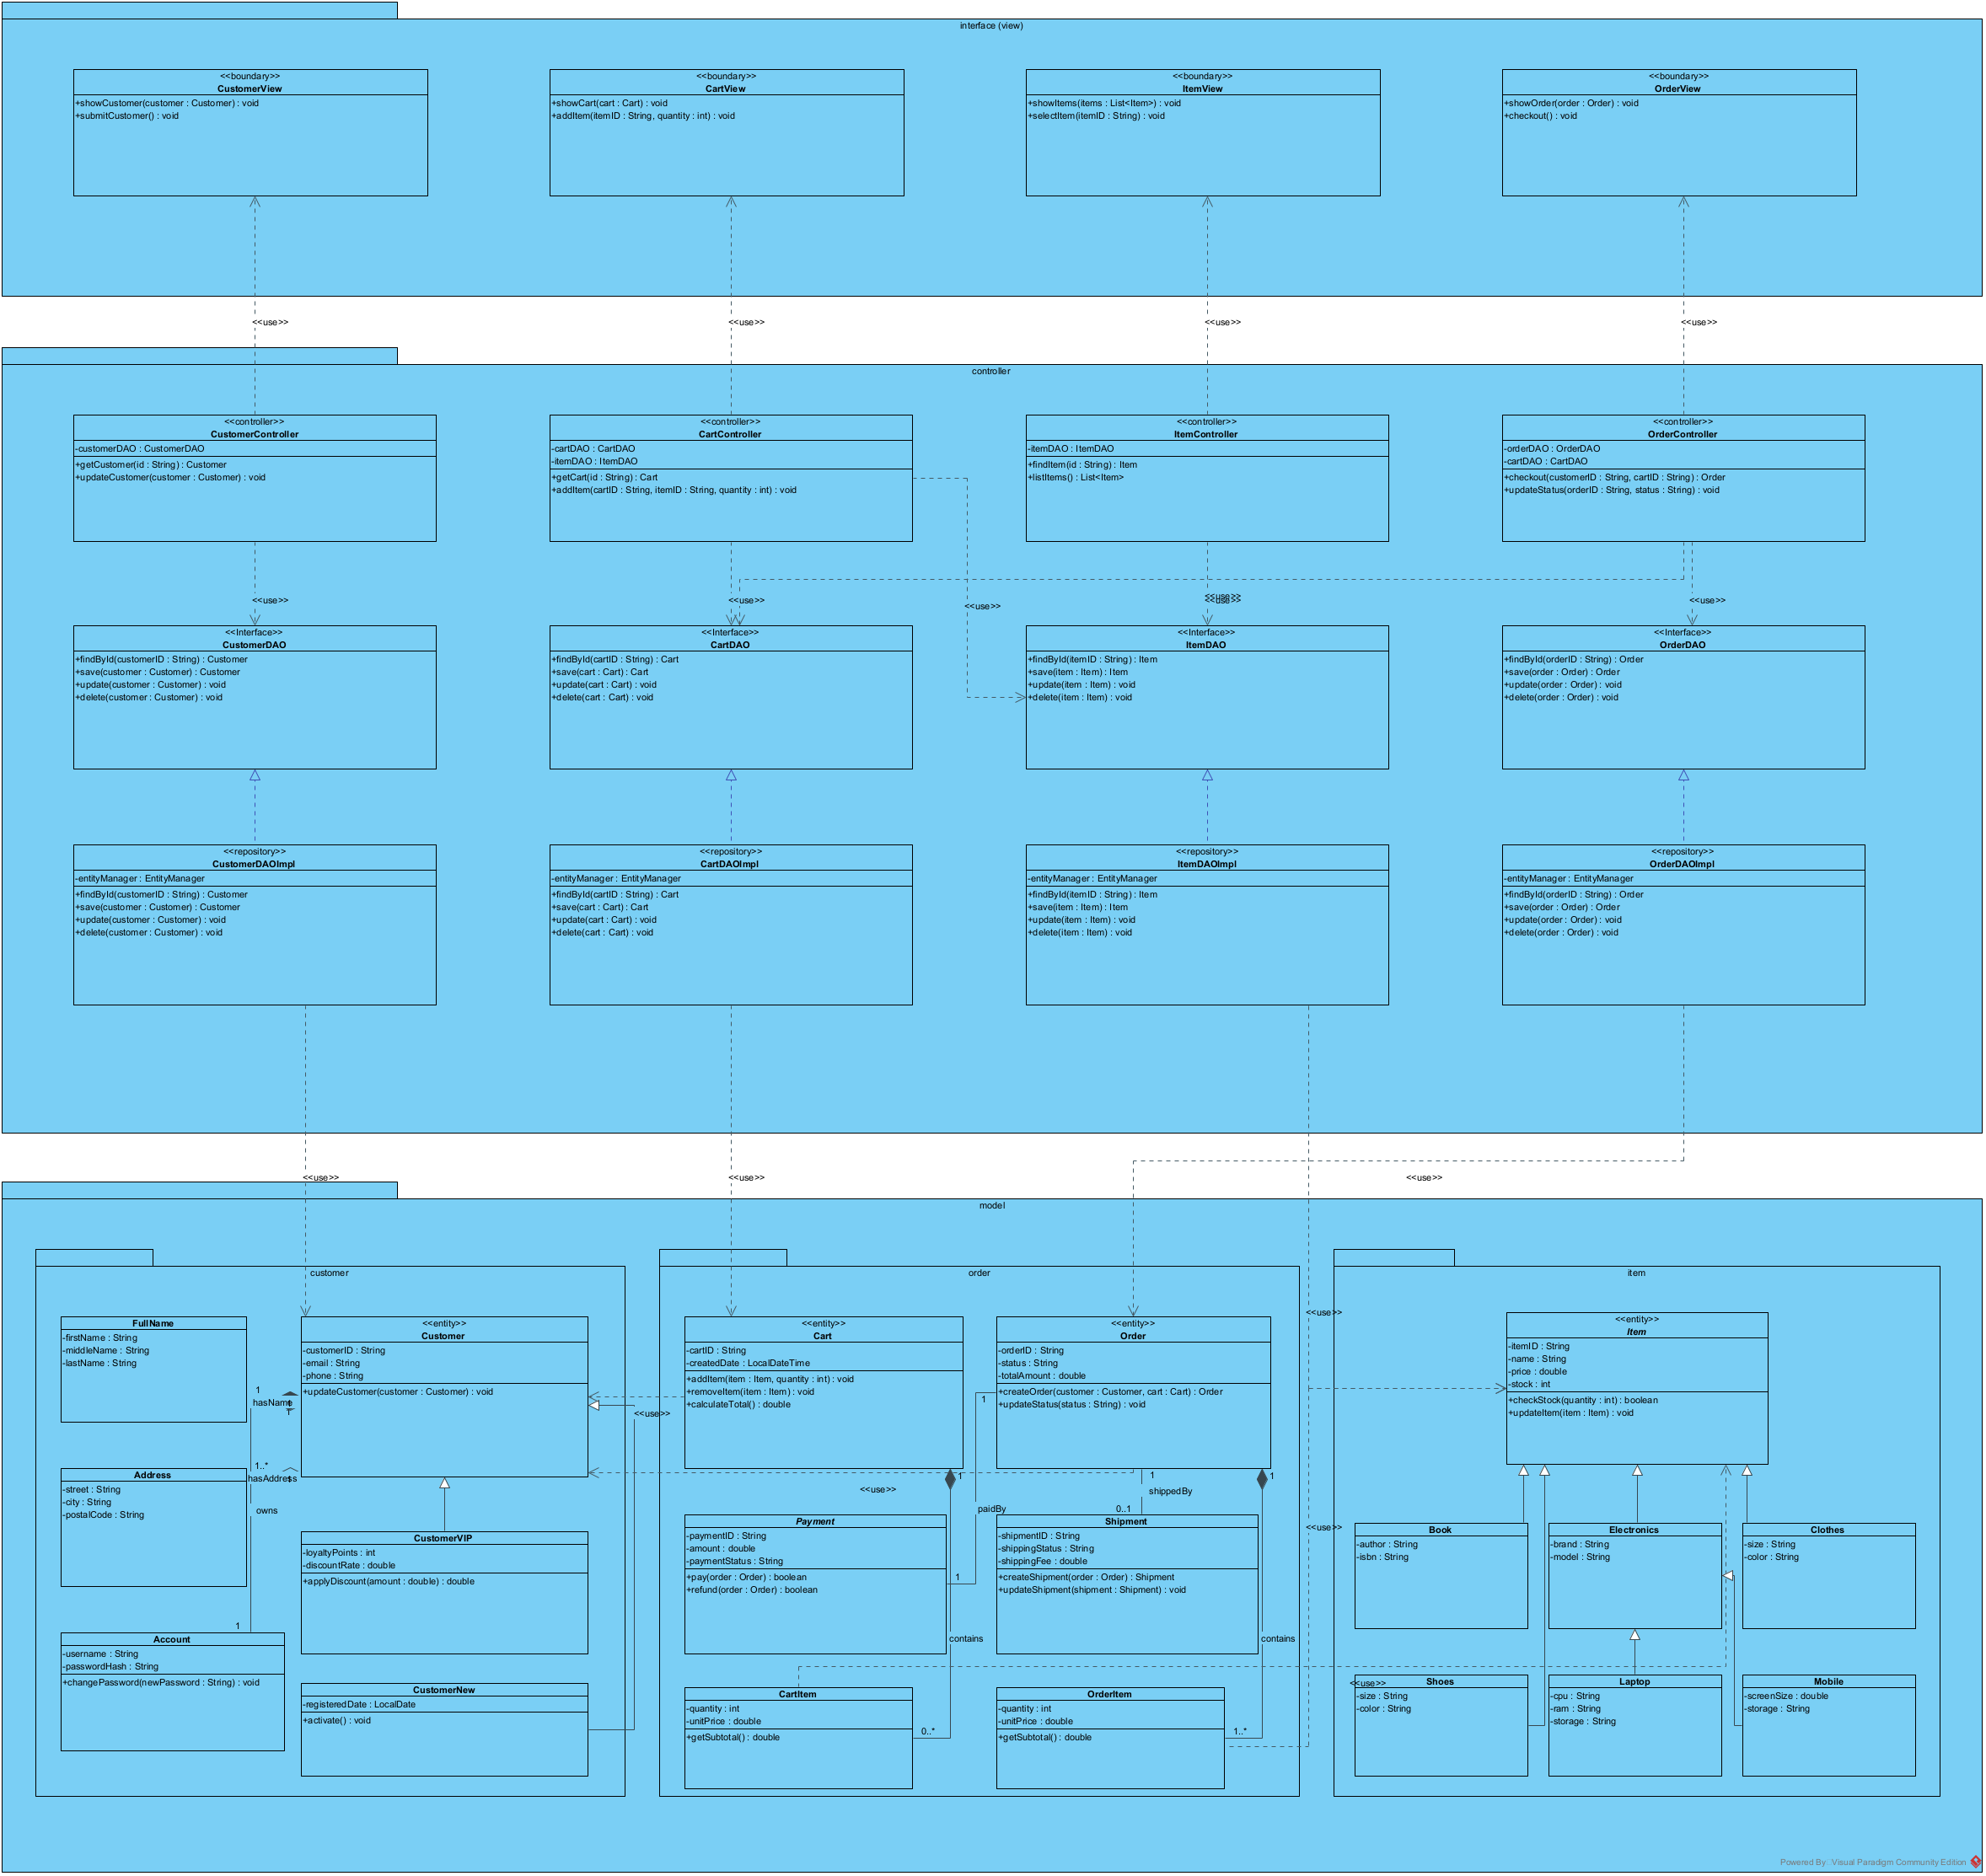
\includegraphics[width=1.17\textwidth,height=0.85\textheight,keepaspectratio]{assets/eComDesign_FINAL_MVC.png}}
\caption{Final MVC and DAO class design exported from the edited Visual Paradigm project. The complete image can be enlarged in the PDF viewer to inspect class members and dependencies.}
\label{fig:mvc}
\end{figure}
\clearpage

\section{Domain organization}
The customer subpackage contains \texttt{Customer}, \texttt{FullName}, \texttt{Address}, and \texttt{Account}. It also includes \texttt{CustomerVIP} and \texttt{CustomerNew} as specializations of customer behavior or state. This arrangement keeps identity and personal information with the customer domain while allowing a specialized customer type to extend the base class.

The order subpackage contains \texttt{Cart} and \texttt{CartItem}, \texttt{Order} and \texttt{OrderItem}, and the associated \texttt{Payment} and \texttt{Shipment} classes. A cart is mutable preparation for a purchase; an order records the placed purchase. Keeping their item classes distinct allows an order line to retain order-time quantity and price rather than depending only on the current state of a cart or catalog item. The handout explicitly places order, payment, and shipment concepts together for this design stage~\cite{handout}.

The item subpackage contains the base \texttt{Item} and several catalog specializations, including \texttt{Book}, \texttt{Electronics}, \texttt{Clothes}, \texttt{Shoes}, \texttt{Laptop}, and \texttt{Mobile}. These specializations communicate variations in item attributes. A production design would still need to decide whether inheritance is preferable to category data for each item type; the diagram records the current educational design choice.

\section{Representative interactions}
\begin{enumerate}
\item \textbf{Customer lookup.} A customer-oriented action is coordinated by \texttt{CustomerController}. The controller depends on \texttt{CustomerDAO} for retrieval and updates. The DAO implementation uses a persistence component and returns a \texttt{Customer} for presentation by \texttt{CustomerView}.
\item \textbf{Cart modification.} \texttt{CartController} coordinates cart operations. It uses \texttt{CartDAO} and, where item data is required, \texttt{ItemDAO}. The domain model represents the cart and its \texttt{CartItem} entries, while the view presents the updated state.
\item \textbf{Catalog browsing.} \texttt{ItemController} uses \texttt{ItemDAO} to obtain items for \texttt{ItemView}. Item-specific attributes remain in the model instead of being embedded in the view.
\item \textbf{Checkout.} \texttt{OrderController} coordinates the transition from cart data to an \texttt{Order} and uses the relevant DAO contracts. \texttt{Payment} and \texttt{Shipment} are associated domain concepts. The diagram defines their class responsibilities but does not itself specify an atomic checkout transaction, payment authorization sequence, or shipping provider protocol.
\end{enumerate}

These paths describe intended responsibilities. They are consistent with the dependency and realization structure visible in Figure~\ref{fig:mvc}, but a class diagram alone cannot prove the order of runtime messages. A sequence diagram and executable tests would be needed for that purpose.

\chapter{Evaluation and Limitations}
\section{Structural verification}
The edited project retained all five class diagrams and the existing model elements. The final MVC diagram contains 35 class shapes. A bounds check found no pair of class rectangles overlapping within the same package, and the diagram's connector endpoints refer to existing diagram elements. The SQLite container passed its integrity check, and Visual Paradigm exported Figure~\ref{fig:mvc} from the edited project. These are reproducible checks of file structure, layout, and diagram export.

\begin{table}[htbp]
\centering
\caption{Verification of the delivered design artifact.}
\begin{tabularx}{\textwidth}{@{}p{53mm}Y@{}}
\toprule
Check & Observed result \\
\midrule
Project database integrity & SQLite integrity check returned \texttt{ok}. \\
Diagram preservation & Five diagrams remained in the project. \\
Final-diagram class layout & 35 class shapes; zero overlaps within the same package. \\
Connector references & No broken diagram-element endpoint references detected. \\
Visual Paradigm export & PNG generated from the edited \texttt{eComDesign.vpp}. \\
\bottomrule
\end{tabularx}
\end{table}

\section{Interpretive limits and further work}
The diagram supports a reasoned architectural review; it is not a running system. In particular, interface signatures do not establish input validation, transaction boundaries, error handling, concurrent inventory reservation, payment security, or persistence mapping. Further work would define those contracts precisely, map classes to a Spring implementation, and test representative workflows. A sequence diagram for checkout would be especially useful because it could specify the temporal relationship among cart validation, order creation, payment, and shipment scheduling.

\chapter{Conclusion}
The final artifact expresses a clear progression from domain analysis to software design. Views, controllers, DAO contracts, repository implementations, and domain classes have distinct roles, while the customer, cart, order, and item areas remain traceable to the original e-commerce concepts. The revised layout makes the three-tier architecture and four functional controller columns easier to compare. Structural checks and a successful Visual Paradigm export support the integrity of the delivered UML artifact; implementation and runtime validation remain separate follow-on activities.

\begin{thebibliography}{9}
\bibitem{handout} Course handout, \textit{From Analysis to Design} (\textit{Từ Phân Tích Đến Thiết Kế}), four-page assignment PDF supplied for Information Systems Analysis and Design.
\bibitem{artifact} V. D. Hieu, \textit{eComDesign.vpp}, Visual Paradigm class-diagram project and exported MVC design image, September 2026.
\end{thebibliography}
\end{document}
